\documentclass{beamer}
\usetheme[nofirafonts]{focus}

% Figures
\usepackage{tikzit}
\input{./figures/styles.tikzstyles}
\usepackage{graphicx, verbatim, listings}
\graphicspath{ {./figures/} }


% Title page details
\title[Markov Chains]{Markov Chains}
\subtitle{Website Traffic Prediction}
\institute{Tanay Biradar}
\date{\today}

\begin{document}

\begin{frame}
  \titlepage
\end{frame}

\begin{frame}
  \frametitle{Website Traffic and PageRank}
  \begin{itemize}
    \item Search engines use popularity to rank pages
    \item Popularity can be quantified by links to a page
      \begin{itemize}
        \item Works in theory, can be abused in practice
      \end{itemize}
    \item Google used a Markov Model (PageRank) to rank popularity
      \begin{itemize}
        \item We're looking to predict traffic, but a similar process applies
      \end{itemize}
  \end{itemize}
\end{frame}

\begin{frame}
  \frametitle{Central Question}
  Which page is a user most likely to land on after starting on a given page?
\end{frame}

\begin{frame}
  \frametitle{Model}
  \begin{itemize}
    \item Represent the internet as a directed graph
        \begin{itemize}
          \item We're looking at a small slice of the web
          \item Assume more links to a page means more likely to land on it
        \end{itemize}
    \item Edges are links, vertices are web pages
        \begin{itemize}
          \item Assume equal probability of traversing every link such that
            \footnote{https://en.wikipedia.org/wiki/PageRank}
            $\Sigma w_{out} = 1$, where $w$ is the edge weight
            \begin{itemize}
              \item The probabilities coming out of every website must sum to 1
            \end{itemize}
        \end{itemize}
  \end{itemize}

  \ctikzfig{internet_graph}
\end{frame}

\begin{frame}
  \frametitle{Data}
  The most complex part is by far the data collection
  \begin{itemize}
    \item Perform BFS to make an adjacency list of the internet
      \begin{itemize}
        \item Keep track of visited nodes to avoid duplicate processing
      \end{itemize}
  \item Stop after storing 2000 links
      \begin{itemize}
        \item I don't have the computing power of Google
      \end{itemize}
  \end{itemize}

  \ctikzfig{internet_graph}
\end{frame}

\begin{frame}
  \frametitle{Data (cont'd)}  
  Adjacency list $A$ stores links between pages \\
  If $A_{ij} = 1$, there is a link from page $i$ to page $j$
  $$
    A = 
    \begin{bmatrix}
    a_{00} & \dots & a_{0n}\\ 
    \vdots & \ddots & \vdots \\ 
    a_{n0} & \dots & a_{nn} 
    \end{bmatrix}
  $$
  Normalize the adjacency list to satisfy $\forall i \  \Sigma w_{out} = \Sigma_j w_i = 1$ \\
  We now have a transition matrix $T$ with probabilities!
\end{frame}


\begin{frame}
  \frametitle{Data (cont'd 2)}
  We can only work with rows/column numbers for the transition matrix \\
  Solution: Map website URLs to unique IDs
  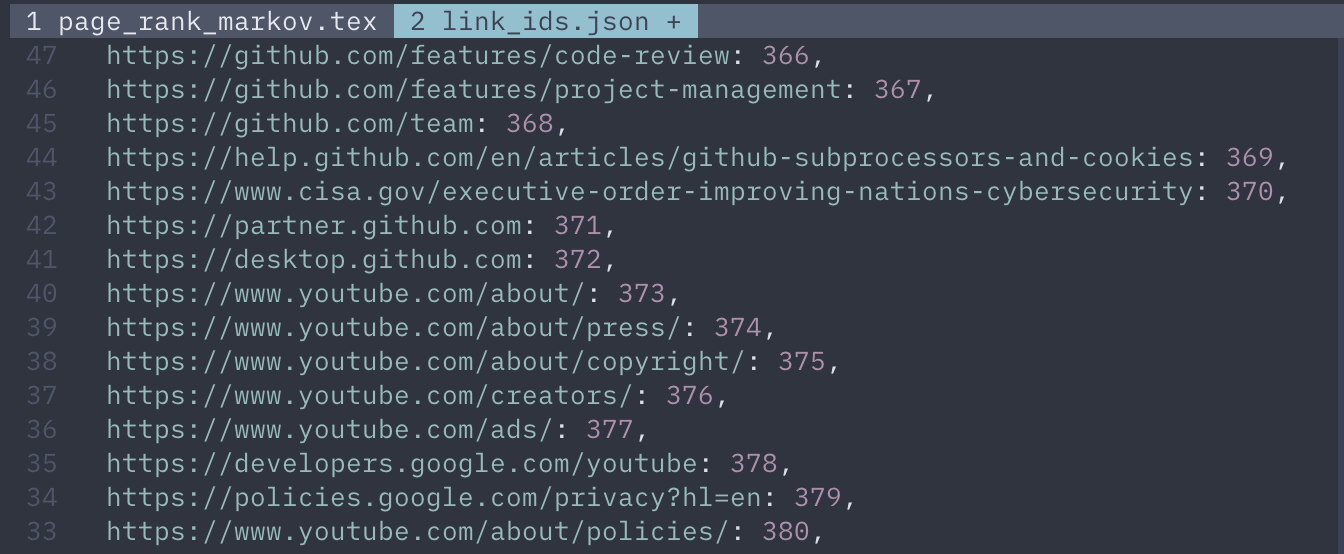
\includegraphics[scale=0.45]{link_ids_json}
\end{frame}

\begin{frame}
  \frametitle{Benchmarking}
  \begin{itemize}
    \item Create a state vector
      \begin{itemize}
        \item Create a 0 vector with same number of dimensions as rows in $T$ \\
        \item Start at a given page, use lookup table to make the corresponding entry 1
          (web page visits are discrete)
      \end{itemize}
    \item Transition matrix is not diagonalizable
      \begin{itemize}
        \item We must simulate and let the state vector converge
      \end{itemize}
  \end{itemize}
\end{frame}

\begin{frame}
  \frametitle{Benchmarking (cont'd)}
  Steps for simulation
  \begin{enumerate}
    \item Multiply transition matrix by state vector
    \item Take web page the user has the greatest probability of landing on and
      set the state vector probability of that page to 1, all others to 0
      \begin{enumerate}
        \item Web page visits are discrete
      \end{enumerate}
    \item Repeat 1-2 either to satisfaction or to convergence
  \end{enumerate}
\end{frame}

\begin{frame}
  \frametitle{Results}
\end{frame}

\end{document}
